% !Mode:: "TeX:UTF-8"
\documentclass[aspectratio=169,12pt]{beamer}

% 主题设置
\usetheme{Madrid}
\usecolortheme{seahorse}

% 中文支持
\usepackage{xeCJK}
\usepackage{fontspec}
\setCJKmainfont{Noto Sans CJK SC}
\setmainfont{Liberation Serif}

% 数学符号
\usepackage{amsmath,amssymb,amsthm}

% 图形支持
\usepackage{graphicx}
\usepackage{tikz}

% 表格
\usepackage{booktabs}
\usepackage{array}
\usepackage{multirow}

% 算法
\usepackage{algorithm}
\usepackage{algorithmic}

% 其他包
\usepackage{xcolor}
\usepackage{hyperref}

% 自定义颜色(常见Beamer学术蓝灰配色)
\definecolor{hitblue}{RGB}{0,63,114}
\definecolor{hitgray}{RGB}{74,85,104}

% 统一Beamer配色
\setbeamercolor{structure}{fg=hitblue}
\setbeamercolor{palette primary}{fg=white,bg=hitblue}
\setbeamercolor{palette secondary}{fg=white,bg=hitgray}
\setbeamercolor{frametitle}{fg=white,bg=hitblue}
\setbeamercolor{title}{fg=white}

\setbeamercolor{block title}{fg=white,bg=hitblue}
\setbeamercolor{block body}{fg=black,bg=hitblue!6}
\setbeamercolor{alertblock title}{fg=white,bg=hitgray}
\setbeamercolor{alertblock body}{fg=black,bg=hitgray!10}
\setbeamercolor{exampleblock title}{fg=white,bg=hitblue!85!black}
\setbeamercolor{exampleblock body}{fg=black,bg=hitblue!8}
\setbeamercolor{alerted text}{fg=hitgray}

% 标题页信息
\title[人脸识别系统隐私攻击研究]{面向人脸识别模型的逆向重建方法研究}
\subtitle{硕士学位论文答辩}
\author[俞磊]{俞磊}
\institute[HIT]{哈尔滨工业大学\\网络空间安全学院}
\date{\today}

% 自定义命令
% 字体大小选项(从大到小):
% \Huge > \huge > \LARGE > \Large > \large > \normalsize(默认)> \small > \footnotesize > \scriptsize > \tiny

% 重定义粗体命令为学术蓝色
\renewcommand{\textbf}[1]{\textcolor{hitblue}{\bfseries #1}}

\newcommand{\highlight}[1]{\textcolor{hitblue}{\textbf{#1}}}
\newcommand{\important}[1]{\textcolor{hitgray}{\textbf{#1}}}

\begin{document}

% 标题页
\begin{frame}[plain]
\titlepage
\end{frame} % 标题页

% 目录
\begin{frame}{目录}
\begin{enumerate}
  \item[\textcolor{hitblue}{1.}] \textbf{研究背景与威胁建模}
  \begin{itemize}
    \item[-] 人脸系统安全威胁与攻击面分析
    \item[-] TIA与MIA核心技术挑战
  \end{itemize}

  \item[\textcolor{hitblue}{2.}] \textbf{研究内容与主要方法}
  \begin{itemize}
    \item[-] 角度约束对比学习的模板逆向设计
    \item[-] 换脸先验迁移的模型反演设计
  \end{itemize}

  \item[\textcolor{hitblue}{3.}] \textbf{TIA方法设计与实验验证}
  \begin{itemize}
    \item[-] 方法架构、训练策略与实验分析
  \end{itemize}

  \item[\textcolor{hitblue}{4.}] \textbf{MIA方法设计与实验验证}
  \begin{itemize}
    \item[-] 三阶段训练、多目标优化与性能评估
  \end{itemize}

  \item[\textcolor{hitblue}{5.}] \textbf{研究结论与防御措施}
  \begin{itemize}
    \item[-] 主要发现总结与防御建议
  \end{itemize}
\end{enumerate}
\end{frame} % 目录

\section{研究背景与意义}

\begin{frame}{研究背景}
\begin{itemize}
\item \highlight{人脸识别进入大规模安全敏感场景}
  \begin{itemize}
  \item 身份认证、公共安全、支付与门禁等关键基础设施
  \item 深度模型显著提升识别性能,同时扩大隐私暴露面
  \end{itemize}

\vspace{0.5em}

\item \highlight{两类系统对应两类核心攻击面}
  \begin{itemize}
  \item 检索型系统:模板泄露引发模板逆向攻击(TIA)
  \item 分类型系统:输出暴露引发模型反演攻击(MIA)
  \end{itemize}

\vspace{0.5em}

\item \highlight{研究问题}
  \begin{itemize}
  \item 如何在身份一致性、视觉真实性与优化稳定性之间实现协同
  \item 如何系统评估两类攻击在真实人脸系统中的隐私风险
  \end{itemize}
\end{itemize}
\end{frame} % 研究背景

\begin{frame}{主要威胁与挑战}
\begin{columns}
\begin{column}{0.5\textwidth}
\textbf{模板逆向攻击 (TIA)}
\begin{itemize}
\item \important{攻击目标:}特征模板
\item \important{攻击场景:}模板库泄露/内部访问滥用
\item \important{攻击方式:}特征嵌入 $\rightarrow$ 人脸图像重建
\item \important{技术挑战:}
  \begin{itemize}
  \item 连续高维特征空间的条件引导
  \item 超球面几何约束下的身份对齐
  \item 感知质量与匹配精度的动态平衡
  \end{itemize}
\end{itemize}
\end{column}

\begin{column}{0.5\textwidth}
\textbf{模型反演攻击 (MIA)}
\begin{itemize}
\item \important{攻击目标:}分类模型
\item \important{攻击场景:}置信度/梯度信息可被查询
\item \important{攻击方式:}类别标签/输出分布 $\rightarrow$ 样本重建
\item \important{技术挑战:}
  \begin{itemize}
  \item 离散标签到连续身份嵌入映射
  \item 模态迁移训练稳定性(图像条件到标签条件)
  \item 攻击准确率与生成保真度协同优化
  \end{itemize}
\end{itemize}
\end{column}
\end{columns}
\end{frame} % 主要威胁与挑战
\section{研究内容与方法}

\begin{frame}{研究内容概述}
\begin{center}
\begin{tikzpicture}[
  box/.style={rectangle, draw, fill=hitblue!10, text width=3.5cm, text centered, minimum height=1.5cm},
  arrow/.style={->, thick, hitblue}
]

\node[box] (tia) at (0,3) {\textbf{模板逆向攻击}\\(TIA)\\检索型系统};
\node[box] (mia) at (0,1) {\textbf{模型反演攻击}\\(MIA)\\分类型系统};

\node[box] (method1) at (5,3) {\textbf{EDM先验 + 角度约束}\\任务不确定性加权\\模板条件梯度引导};
\node[box] (method2) at (5,1) {\textbf{换脸先验迁移}\\标签条件嵌入 + LoRA\\三阶段渐进训练};

\node[box] (result) at (10,2) {\textbf{系统评估}\\攻击有效性与保真度\\防御启示};

\draw[arrow] (tia) -- (method1);
\draw[arrow] (mia) -- (method2);
\draw[arrow] (method1) -- (result);
\draw[arrow] (method2) -- (result);

\end{tikzpicture}
\end{center}

\vspace{0.5em}

\textbf{研究目标:}针对检索型与分类型人脸识别系统,分别构建TIA与MIA方法并进行系统化风险评估
\end{frame} % 研究内容概述

\begin{frame}{主要研究方法}
\small
\begin{block}{模板逆向攻击(TIA)涉及工作}
\begin{itemize}
\item \highlight{EDM生成建模:}学习特征模板到人脸图像的条件逆映射
\item \highlight{角度约束对比学习:}在超球面空间强化身份判别与特征对齐
\item \highlight{两阶段训练+模板引导推理:}结合任务不确定性加权与梯度引导采样
\end{itemize}
\end{block}

\begin{block}{模型反演攻击(MIA)涉及工作}
\begin{itemize}
\item \highlight{换脸先验迁移:}复用身份-属性解耦先验提升重建真实性
\item \highlight{标签条件嵌入:}建立离散类别到连续身份嵌入的可学习映射
\item \highlight{LoRA与多目标优化:}采用三阶段渐进训练实现稳定模态迁移
\end{itemize}
\end{block}


\end{frame} % 主要研究方法

\section{基于角度约束对比学习的模板逆向攻击}

\subsection{TIA方法:基于扩散模型的角度约束对比学习}

\begin{frame}{TIA问题定义与关键挑战}
\begin{block}{攻击目标}
给定泄露模板 $t=F(x_0)$,生成重建图像 $\hat{x}$,同时满足身份一致性与视觉真实性。
\end{block}

\begin{columns}[T]
\column{0.5\textwidth}
\textbf{形式化目标}
\begin{equation*}
\hat{x}=\arg\min_x\,\mathcal{L}_{embed}(F(x),t)+\lambda_{perc}\mathcal{L}_{perc}(x)
\end{equation*}

\column{0.5\textwidth}
\textbf{关键挑战}
\begin{itemize}
  \item 降维映射多对一,逆问题欠定
  \item ArcFace超球面几何与欧式优化失配
  \item 感知质量与身份匹配目标冲突
\end{itemize}
\end{columns}
\end{frame} % TIA问题定义与关键挑战

\begin{frame}{TIA方法架构}
\begin{figure}
  \centering
  \includegraphics[width=0.83\textwidth]{figures/train_finetune.pdf}
  \caption{基于扩散模型的TIA方法架构}
\end{figure}

\begin{itemize}
  \item \textbf{生成主干:}EDM去噪网络,保证样本位于自然人脸流形附近
  \item \textbf{特征监督:}ArcFace提取身份特征,构建角度约束匹配目标
  \item \textbf{优化框架:}任务不确定性加权 + 类内多样性正则
\end{itemize}
\end{frame} % TIA方法架构

\begin{frame}{TIA损失函数设计}
\small
\begin{columns}[T]
  \column{0.5\textwidth}
  \textbf{核心损失项}
  \begin{itemize}
    \item 像素去噪损失 $\mathcal{L}_{pixel}$
    \item 角度约束特征损失 $\mathcal{L}_{feat}$
    \item 类内多样性损失 $\mathcal{L}_{div}$
  \end{itemize}

  \textbf{角度约束特征损失}
  \begin{equation*}
  \mathcal{L}_{feat}=\max(0,m+\cos(F(\hat{x}),F(x_{neg}))-\cos(F(\hat{x}),F(x_0)))
  \end{equation*}

  \column{0.5\textwidth}
  \textbf{总体优化目标}
  \begin{equation*}
  \mathcal{L}=\frac{1}{2\sigma_p^2}\mathcal{L}_{pixel}+\frac{1}{2\sigma_f^2}\mathcal{L}_{feat}
  +\frac{1}{2}(\log\sigma_p^2+\log\sigma_f^2)-\beta\mathcal{L}_{div}
  \end{equation*}

  \begin{itemize}
    \item $\sigma_p,\sigma_f$为可学习不确定性参数
    \item 训练中自适应平衡生成质量与攻击有效性
  \end{itemize}
\end{columns}
\end{frame} % TIA损失函数设计

\begin{frame}{TIA训练与推理策略}
\small
\textbf{两阶段训练策略}
\begin{columns}
\begin{column}{0.5\textwidth}
\textbf{阶段1:预热阶段}
\begin{itemize}
\item 仅优化 $\mathcal{L}_{pixel}$
\item 建立稳定去噪与人脸结构先验
\end{itemize}

\textbf{阶段2:主训练阶段}
\begin{itemize}
\item 启用完整混合损失
\item 联合更新网络参数与$\sigma_p,\sigma_f$
\end{itemize}
\end{column}

\begin{column}{0.5\textwidth}
\textbf{推理阶段:模板条件梯度引导}
\begin{equation*}
x_{i-1}=x_i+(\sigma_{i-1}-\sigma_i)
\left[d_{base}+\alpha\nabla_{x_i}\mathrm{sim}(F(x_i),t)\right]
\end{equation*}

\begin{itemize}
\item 通过模板梯度动态修正采样轨迹
\item 在保证视觉真实性前提下提升特征匹配精度
\item 与训练目标形成一致闭环
\end{itemize}
\end{column}
\end{columns}
\end{frame} % TIA训练与推理策略

\section{TIA实验结果与分析}

\begin{frame}{TIA实验设置与评估指标}
\begin{columns}[T]
\column{0.5\textwidth}
\textbf{实验设置}
\begin{itemize}
  \item 训练集:CelebA(202,599)
  \item 测试集:MOBIO、LFW、AgeDB、IJB-C
  \item 目标识别器:ArcFace(512维归一化模板)
  \item 白盒攻击设定:可访问目标模型参数与梯度
\end{itemize}

\column{0.5\textwidth}
\textbf{评估指标}
\begin{itemize}
  \item 攻击成功率:SAR@FMR=$10^{-2},10^{-3}$
  \item 生成质量:FID(越低越好)
  \item 身份保持:ID-Pres(越高越好)
\end{itemize}

\textbf{对比方法}
\begin{itemize}
  \item NBNet、Vendrow、GaFaR、Shahreza等代表方法
\end{itemize}
\end{columns}
\end{frame} % TIA实验设置与评估指标

\begin{frame}{TIA实验结果}
\begin{table}
\centering
\footnotesize
\caption{TIA方法定量性能对比(LFW测试集)}
\vspace{-0.2cm}
\begin{tabular}{lcccc}
\toprule
\textbf{方法} & \textbf{SAR@10$^{-2}$} & \textbf{SAR@10$^{-3}$} & \textbf{FID↓} & \textbf{身份保持度↑} \\
\midrule
NBNetB-P & 61.53\% & 40.18\% & 52.4 & 0.703 \\
Vendrow et al. & 77.15\% & 57.84\% & 41.2 & 0.768 \\
GaFaR & 89.41\% & 79.97\% & 32.1 & 0.834 \\
Shahreza et al. & 92.47\% & 85.14\% & 28.5 & 0.891 \\
\midrule
\textbf{本文方法} & \textbf{94.23\%} & \textbf{84.23\%} & \textbf{18.27} & \textbf{0.947} \\
\bottomrule
\end{tabular}
\end{table}

\vspace{-0.1cm}
\begin{block}{关键发现}
\begin{itemize}
  \item 在LFW上,SAR@10$^{-2}$提升\textbf{2.76\%},FID降低\textbf{35.9\%}
  \item SAR@10$^{-3}$略低于Shahreza et al.(84.23\% vs 85.14\%),但FID与ID-Pres更优
\end{itemize}
\end{block}
\end{frame} % TIA实验结果

\begin{frame}{TIA方法跨数据集性能表现}
\begin{table}
\centering
\scriptsize
\caption{TIA方法在不同数据集上的攻击成功率对比}
\vspace{-0.2cm}
\begin{tabular}{lcccc}
\toprule
\textbf{方法} & \textbf{MOBIO} & \textbf{LFW} & \textbf{AgeDB} & \textbf{IJB-C} \\
\midrule
\multicolumn{5}{c}{\textbf{FMR=$10^{-2}$}} \\
\midrule
Vendrow et al. & 69.38 & 77.15 & 44.62 & 38.51 \\
GaFaR & 95.84 & 89.41 & 63.45 & 69.32 \\
Shahreza et al. & 96.53 & 92.47 & 73.91 & 78.62 \\
\textbf{本文方法} & \textbf{97.38} & \textbf{94.23} & \textbf{75.64} & \textbf{82.91} \\
\midrule
\multicolumn{5}{c}{\textbf{FMR=$10^{-3}$}} \\
\midrule
Vendrow et al. & 29.18 & 57.84 & 29.78 & 7.56 \\
GaFaR & 82.93 & 79.97 & 49.08 & 29.91 \\
Shahreza et al. & 84.89 & 85.14 & 60.18 & 45.57 \\
\textbf{本文方法} & \textbf{87.87} & 84.23 & \textbf{65.81} & \textbf{55.58} \\
\bottomrule
\end{tabular}
\end{table}

\begin{block}{关键发现}
\begin{itemize}
  \item \textbf{跨数据集泛化:}MOBIO/AgeDB/IJB-C在两个FMR阈值下均为最优
  \item \textbf{高安全阈值:}FMR=$10^{-3}$下平均攻击成功率达73.41\%
\end{itemize}
\end{block}
\end{frame} % TIA方法跨数据集性能表现

\begin{frame}{TIA训练过程分析}
\begin{figure}
\centering
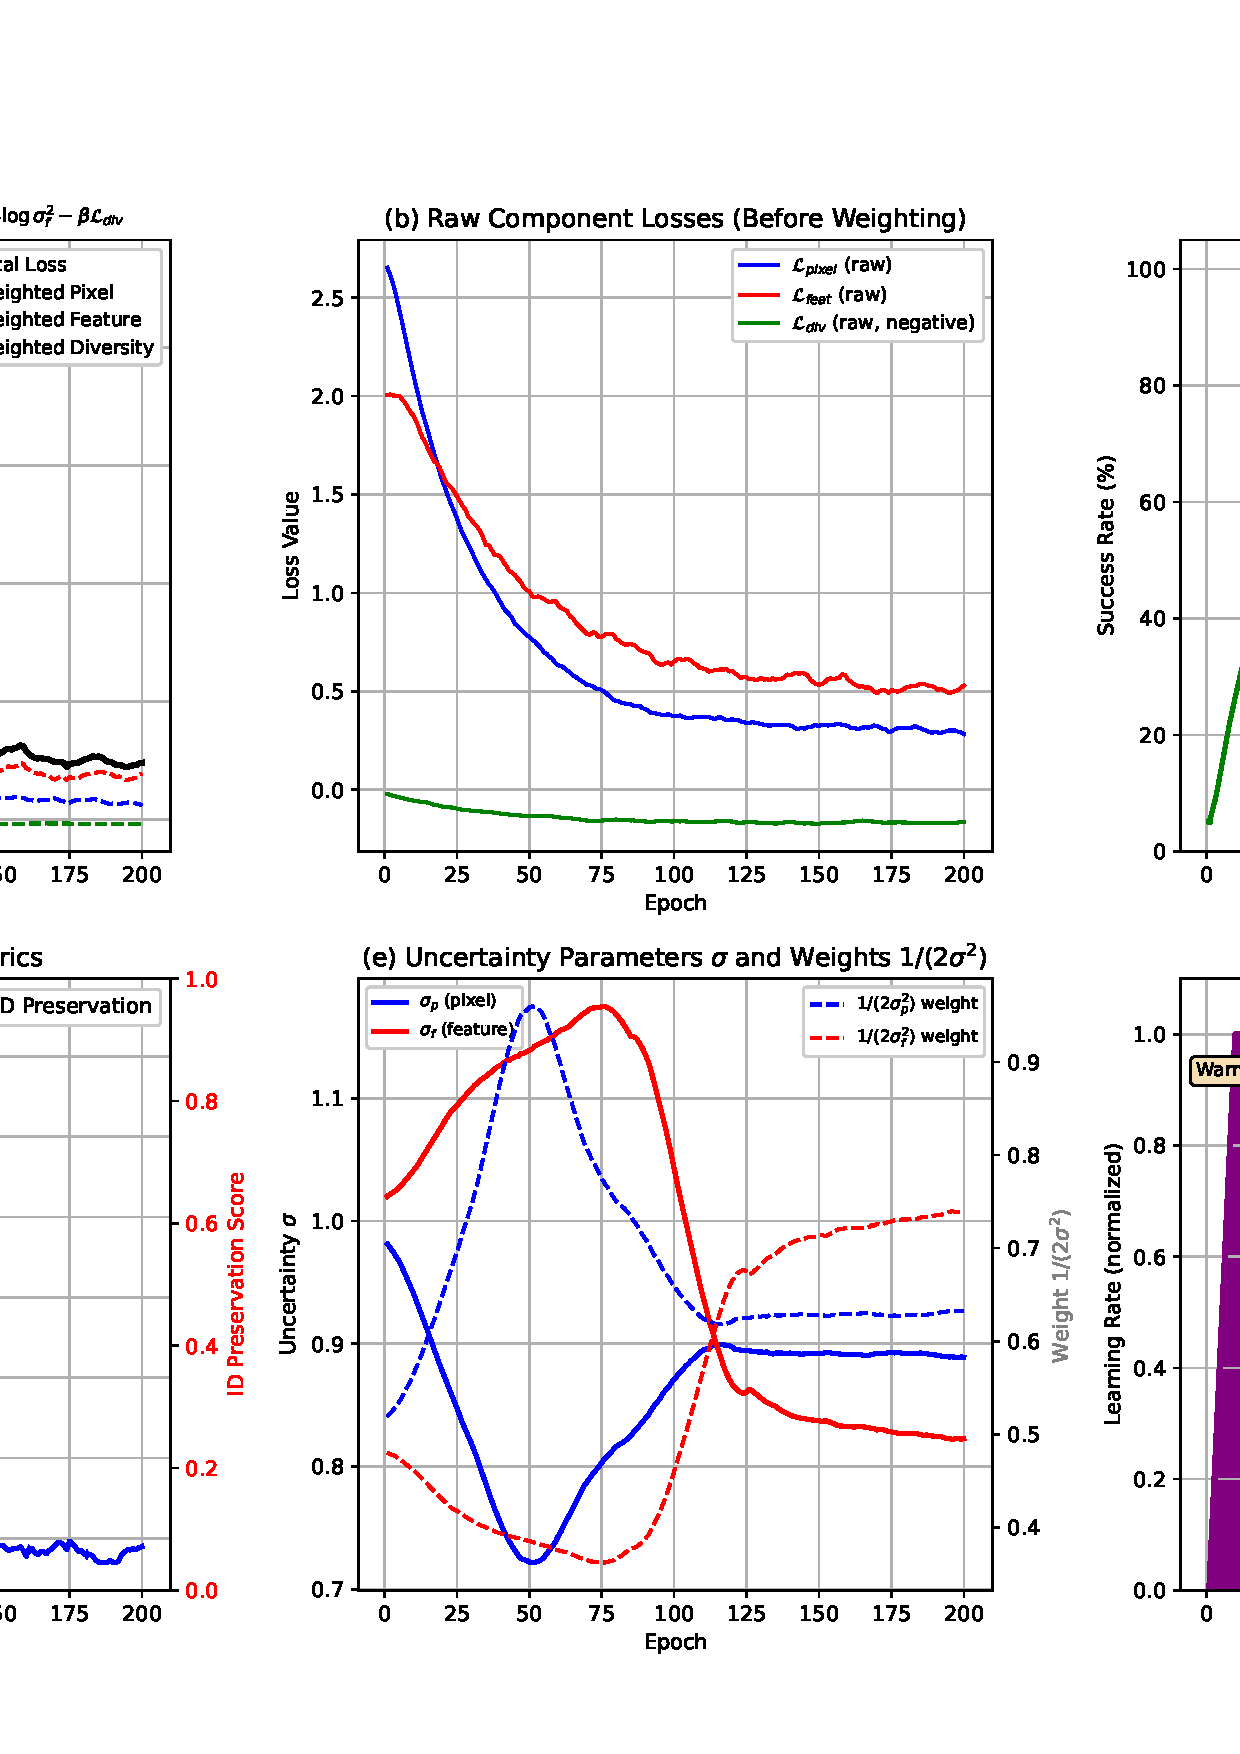
\includegraphics[width=0.95\textwidth]{figures/tia_training_curves.pdf}
\caption{TIA方法训练过程的损失与指标演化曲线}
\end{figure}

\begin{block}{与论文一致的关键信息}
\begin{itemize}
  \item 各项损失与指标整体稳定收敛,SAR上升、FID下降、ID-Pres提升
  \item 不确定性参数$\sigma_p,\sigma_f$自适应演化,训练后期特征匹配任务权重更高
\end{itemize}
\end{block}
\end{frame} % TIA训练过程分析

\begin{frame}{TIA消融实验分析}
\begin{columns}[T]
  \column{0.55\textwidth}
  \begin{table}
  \centering
  \footnotesize
  \caption{TIA模块消融(LFW)}
  \begin{tabular}{lcc}
  \toprule
  \textbf{模型配置} & \textbf{SAR@10$^{-3}$} & \textbf{FID} \\
  \midrule
  仅像素损失 & 41.67\% & 52.46 \\
  +角度约束 & 79.83\% & 32.18 \\
  +任务加权 & 82.17\% & 27.54 \\
  +多样性正则 & 84.23\% & 18.27 \\
  \bottomrule
  \end{tabular}
  \end{table}

  \column{0.4\textwidth}
  \begin{block}{结论}
  \begin{itemize}
    \item 各模块带来渐进收益
    \item 完整模型相对基线提升42.56个百分点
  \end{itemize}
  \end{block}
\end{columns}
\end{frame} % TIA消融实验分析

\section{MIA设计与实验}

\subsection{MIA方法:基于换脸先验的身份嵌入学习}

\begin{frame}{MIA问题定义与核心挑战}
\small
\textbf{目标:}仅给定类别标签$y$,生成样本$\hat{x}$,使其同时满足:
\begin{itemize}
  \item \textbf{攻击有效性:}被目标分类器高置信识别为$y$
  \item \textbf{视觉真实性:}保持自然人脸纹理与结构
\end{itemize}

\begin{block}{核心矛盾(第4章)}
\begin{enumerate}
  \item 换脸模型原生依赖\textbf{目标图像条件},攻击场景只有\textbf{离散标签}
  \item 标签嵌入分布与ArcFace真实身份嵌入分布存在偏移
  \item 分类器攻击目标与生成保真目标需要动态平衡
\end{enumerate}
\end{block}

\begin{alertblock}{一句话结论}
MIA的关键是将“标签条件”稳定迁移到“换脸先验”的身份控制通道。
\end{alertblock}
\end{frame} % MIA问题定义与核心挑战

\begin{frame}{MIA方法架构}
\begin{figure}
  \centering
  \includegraphics[height=0.43\textheight,keepaspectratio]{figures/infer_mia.pdf}
\end{figure}

\begin{itemize}
  \item \textbf{标签条件嵌入层:}$y\rightarrow e_{id}\in\mathbb{R}^{512}$并归一化
  \item \textbf{换脸先验适配:}在冻结主干上引入LoRA低秩增量($r=16,\alpha=32$)
  \item \textbf{目标引导优化:}联合分类器与身份约束端到端训练
\end{itemize}

\begin{alertblock}{一句话结论}
架构核心是“标签嵌入 + LoRA适配 + 多目标优化”的协同。
\end{alertblock}
\end{frame} % MIA方法架构

\begin{frame}{MIA多目标损失设计}
\small
\begin{columns}[T]
  \column{0.52\textwidth}
  \textbf{六类损失(第4章)}
  \begin{itemize}
    \item 扩散先验:$\mathcal{L}_{prior}$
    \item 分类引导(top-k margin):$\mathcal{L}_{cls}$
    \item 特征正则(p-reg):$\mathcal{L}_{p-reg}$
    \item 身份一致性对比:$\mathcal{L}_{id}$
    \item 感知质量(LPIPS):$\mathcal{L}_{perc}$
    \item 嵌入/LoRA正则:$\mathcal{L}_{reg}$
  \end{itemize}

  \column{0.46\textwidth}
  \begin{block}{任务不确定性加权}
  \small
  \[
  \mathcal{L}_{total}=\sum_i\left(\frac{1}{2\sigma_i^2}\mathcal{L}_i+\frac{1}{2}\log\sigma_i^2\right)
  \]
  \normalsize
  自动学习各任务权重,减少人工调参依赖。
  \end{block}
\end{columns}

\begin{alertblock}{一句话结论}
通过自适应加权,MIA在“攻击强度”和“生成质量”之间实现动态平衡。
\end{alertblock}
\end{frame} % MIA多目标损失设计

\begin{frame}{MIA训练与推理策略}
\small
\begin{columns}[T]
  \column{0.52\textwidth}
  \textbf{三阶段渐进训练}
  \begin{enumerate}
    \item 图像条件预热:稳定先验生成能力
    \item 混合条件过渡:余弦退火平滑迁移
    \item 纯标签适配:聚焦分类器攻击与身份对齐
  \end{enumerate}

  \column{0.46\textwidth}
  \textbf{推理阶段}
  \begin{itemize}
    \item 标签嵌入驱动生成
    \item 关键步分类器引导修正采样轨迹
    \item 候选样本按目标置信度筛选
  \end{itemize}
\end{columns}

\begin{block}{论文对应结果}
三阶段训练将TarAcc从70.85\%提升到94.87\%,并同步降低FID到23.26。
\end{block}
\end{frame} % MIA训练与推理策略

\begin{frame}{MIA实验设置与评估指标}
\begin{columns}[T]
  \column{0.52\textwidth}
  \textbf{数据与目标模型}
  \begin{itemize}
    \item 目标任务:VGGFace2(1000类)
    \item 辅助数据:CelebA、FaceScrub
    \item 目标分类器:ArcFace / IR152 / Face.evoLVe
  \end{itemize}

  \textbf{训练配置}
  \begin{itemize}
    \item LoRA: $r=16,\alpha=32$,仅微调少量参数
    \item 优化器:AdamW,LoRA lr=$5\times10^{-6}$
    \item 推理:DDIM 50步
  \end{itemize}

  \column{0.46\textwidth}
  \textbf{评估指标}
  \begin{itemize}
    \item TarAcc:目标分类器命中率
    \item EvalAcc:独立分类器泛化识别率
    \item FID:生成分布质量
    \item KNN Dist:身份特征邻域一致性
  \end{itemize}

  \begin{block}{对比方法}
  GMI、FMI、PLG-MI、Diff-MI
  \end{block}
\end{columns}
\end{frame} % MIA实验设置与评估指标

\begin{frame}{MIA基准性能对比(ArcFace)}
\begin{table}
\centering
\footnotesize
\caption{VGGFace2上MIA方法定量对比}
\begin{tabular}{lcccc}
\toprule
\textbf{方法} & \textbf{TarAcc$\uparrow$} & \textbf{EvalAcc$\uparrow$} & \textbf{FID$\downarrow$} & \textbf{KNN$\uparrow$} \\
\midrule
GMI & 28.52\% & 1.38\% & 24.87 & 0.559 \\
FMI & 31.27\% & 21.63\% & 36.42 & 0.531 \\
PLG-MI & 40.95\% & 16.87\% & 43.26 & 0.579 \\
Diff-MI & 94.18\% & 75.62\% & 29.53 & \textbf{0.743} \\
\midrule
\textbf{本文方法} & \textbf{94.87\%} & \textbf{83.15\%} & \textbf{23.26} & 0.717 \\
\bottomrule
\end{tabular}
\end{table}

\begin{block}{结论}
相较Diff-MI,EvalAcc提升7.53个百分点、FID降低6.27,说明生成样本更具可迁移身份语义与视觉真实性。
\end{block}
\end{frame} % MIA基准性能对比(ArcFace)

\begin{frame}{MIA方法跨架构泛化能力}
\begin{table}
\centering
\tiny
\caption{MIA方法在不同目标分类器架构下的性能}
\vspace{-0.2cm}
\begin{tabular}{lcccc}
\toprule
\textbf{方法} & \textbf{目标准确率} & \textbf{评估准确率} & \textbf{FID} & \textbf{KNN} \\
\midrule
\multicolumn{5}{c}{\textbf{ArcFace分类器}} \\
\midrule
Diff-MI & 94.18\% & 75.62\% & 29.53 & 0.743 \\
\textbf{本文} & \textbf{94.87\%} & \textbf{83.15\%} & \textbf{23.26} & 0.717 \\
\midrule
\multicolumn{5}{c}{\textbf{IR152分类器}} \\
\midrule
Diff-MI & 93.75\% & 76.84\% & 32.68 & 0.818 \\
\textbf{本文} & \textbf{93.28\%} & \textbf{84.23\%} & \textbf{25.83} & \textbf{0.853} \\
\midrule
\multicolumn{5}{c}{\textbf{Face.evoLVe分类器}} \\
\midrule
Diff-MI & 95.42\% & 79.21\% & 36.47 & 0.856 \\
\textbf{本文} & 94.38\% & \textbf{82.94\%} & \textbf{26.91} & \textbf{0.902} \\
\bottomrule
\end{tabular}
\end{table}

\begin{block}{关键发现}
评估准确率均超过82\%,FID性能在所有架构上均优于基线
\end{block}
\end{frame} % MIA方法跨架构泛化能力

\begin{frame}{MIA训练过程分析}
\begin{figure}
\centering
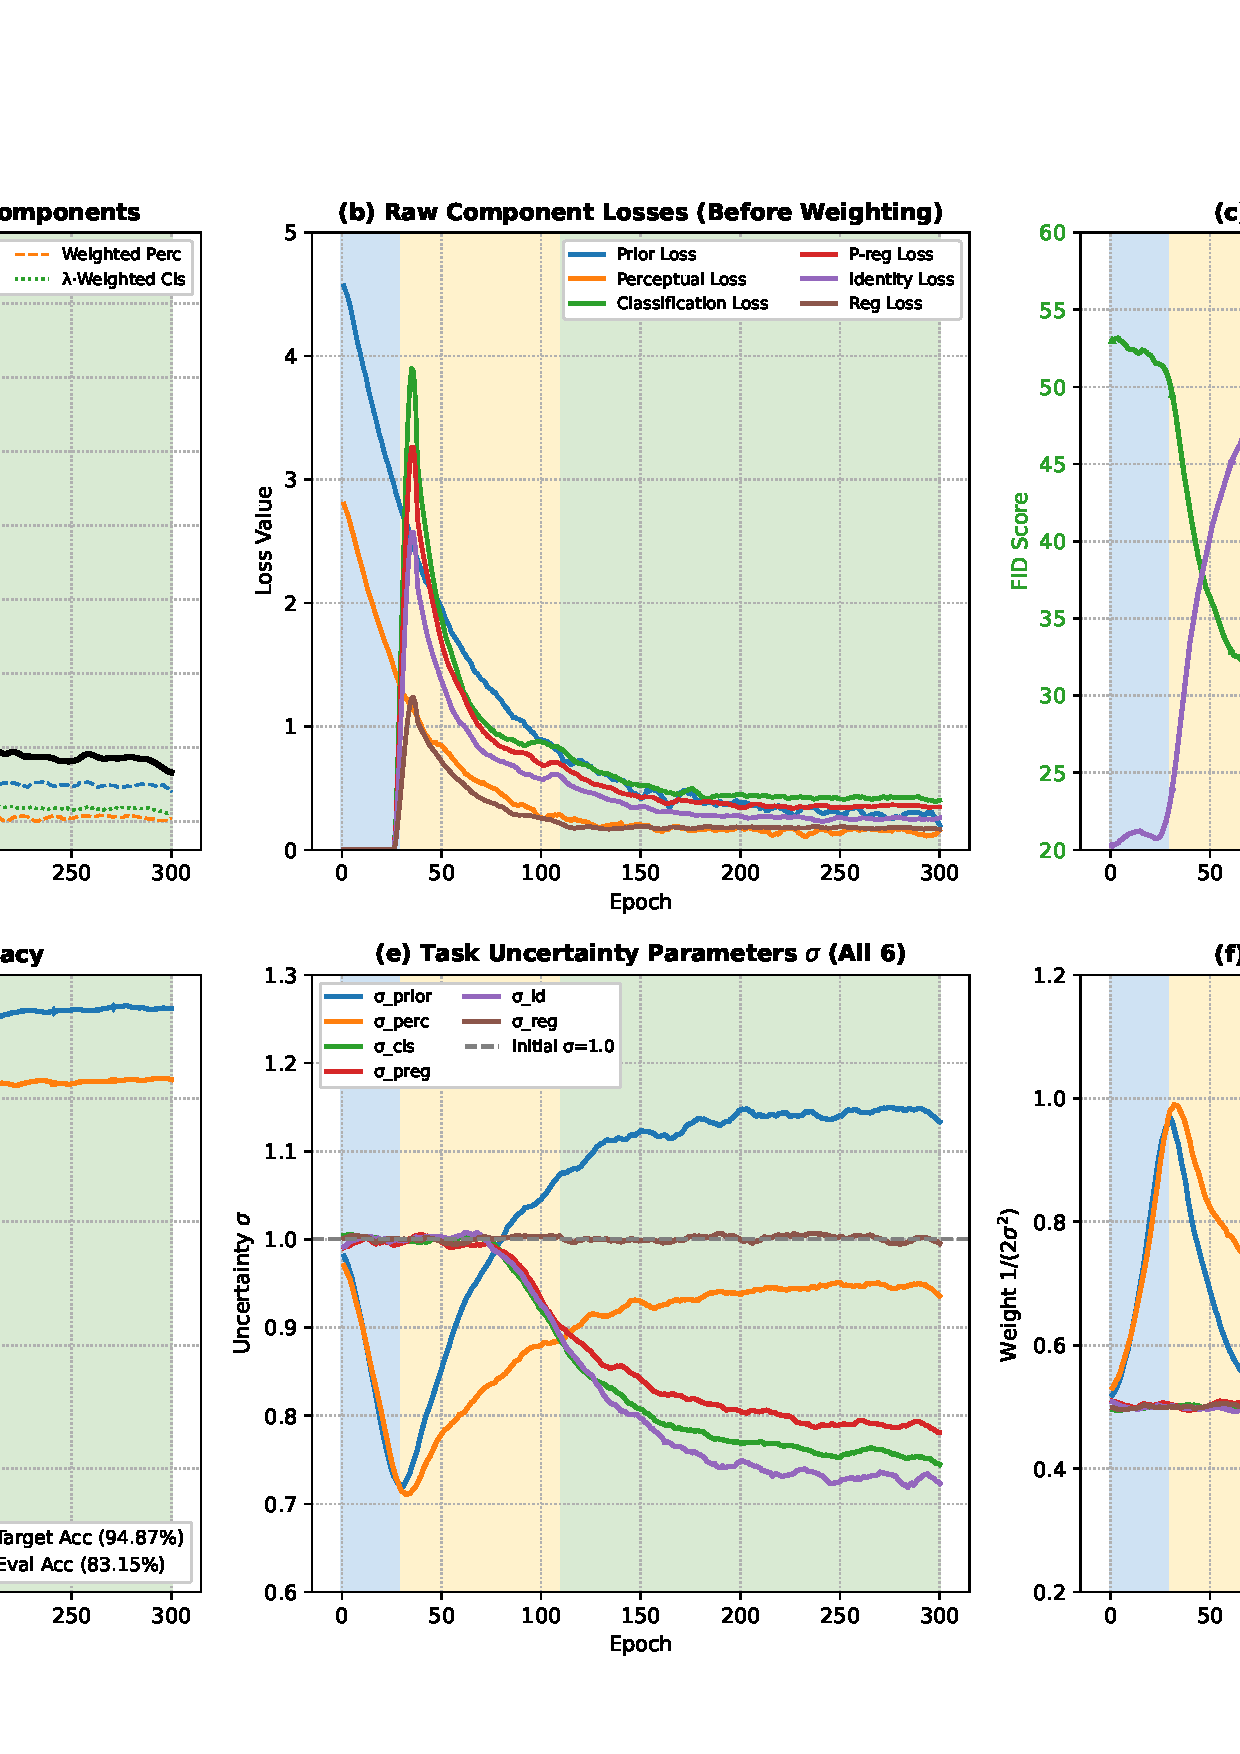
\includegraphics[height=0.47\textheight,keepaspectratio]{figures/mia_training_curves.pdf}
\caption{MIA方法三阶段渐进式训练过程的损失与指标演化曲线}
\end{figure}

\begin{itemize}
  \item 三阶段(预热→过渡→纯标签)下,FID持续下降、KNN与准确率持续提升
  \item 任务不确定性参数与权重系数动态调整,实现多目标自动平衡
\end{itemize}

{\small \textbf{一句话结论:}训练曲线验证“平滑模态迁移 + 自适应权重”是MIA稳定收敛的关键机制。}
\end{frame} % MIA训练过程分析

\begin{frame}{MIA消融实验分析}
\begin{columns}[T]
  \column{0.52\textwidth}
  \begin{table}
  \centering
  \footnotesize
  \caption{训练策略消融}
  \begin{tabular}{lccc}
  \toprule
  \textbf{训练策略} & \textbf{TarAcc} & \textbf{EvalAcc} & \textbf{FID} \\
  \midrule
  单阶段(标签) & 70.85\% & 63.74\% & 43.21 \\
  两阶段训练 & 88.92\% & 78.56\% & 32.45 \\
  三阶段训练 & 94.87\% & 83.15\% & 23.26 \\
  \bottomrule
  \end{tabular}
  \end{table}

  \column{0.45\textwidth}
  \begin{table}
  \centering
  \footnotesize
  \caption{损失组合消融}
  \begin{tabular}{lcc}
  \toprule
  \textbf{损失组合} & \textbf{TarAcc} & \textbf{EvalAcc} \\
  \midrule
  仅扩散先验 & 7.85\% & 5.92\% \\
  +分类引导 & 77.24\% & 70.38\% \\
  +身份一致性 & 92.56\% & 79.47\% \\
  +感知质量 & 94.87\% & 83.15\% \\
  \bottomrule
  \end{tabular}
  \end{table}
\end{columns}

\begin{block}{结论}
三阶段渐进训练与完整损失组合共同决定MIA的攻击精度和生成质量。
\end{block}
\end{frame} % MIA消融实验分析

\section{研究结论}

\begin{frame}{研究总结}
\small

\begin{block}{基于角度约束对比学习的模板逆向重建方法}
\begin{itemize}
  \item 以EDM扩散模型为骨干,设计角度约束对比学习损失,精确对齐超球面决策边界
  \item 任务不确定性加权自动平衡多目标损失,模板条件梯度引导动态调整采样轨迹
  \item MOBIO攻击成功率97.38\%,LFW上FID=18.27
\end{itemize}
\end{block}

\vspace{0.2em}

\begin{block}{基于换脸先验迁移的多目标自适应模型反演方法}
\begin{itemize}
  \item 将扩散换脸模型应用于模型反演,通过标签条件嵌入层建立标签到身份的映射
  \item 渐进三阶段训练+LoRA参数高效微调
  \item 目标准确率94.87\%,评估准确率83.15\%,FID=23.26
\end{itemize}
\end{block}

\end{frame} % 研究总结

\begin{frame}{防御措施讨论}

\textbf{特征空间防御}
\begin{itemize}
\item \textbf{特征混淆:}破坏超球面几何结构,削弱角度约束对比学习的判别能力
\item \textbf{噪声注入:}在特征空间添加随机噪声,降低攻击的特征匹配精度
\end{itemize}

\vspace{0.4em}

\textbf{对抗训练防御}
\begin{itemize}
\item \textbf{对抗样本训练:}使用逆向重建样本对识别器进行对抗训练,提升模型鲁棒性
\item \textbf{正则化约束:}限制模型过度拟合,约束梯度信息的泄露程度
\end{itemize}

\vspace{0.4em}

\textbf{模型输出防御}
\begin{itemize}
\item \textbf{差分隐私机制:}在模型输出中添加校准噪声,干扰梯度信息获取
\item \textbf{置信度限制策略:}限制输出置信度范围,直接降低模型反演攻击有效性
\end{itemize}

\end{frame} % 防御措施讨论





\begin{frame}{专家评议意见及修改}
\footnotesize
\begin{enumerate}
\item  论文结论虽然提到了该成果在高安全阈值下攻击的成功率,但是并未讨论可能的防御手段对本文攻击有效性的影响。模型隐私性在业界获得了很高的关注度,也有若干防御措施提出。可讨论如何防御本文攻击或在有防御策略保护下本文攻击所受的影响。\\
\textcolor{hitblue}{在结论部分增加防御措施讨论}

\item  应规范术语及英文缩写的使用,如未给出"生成对抗网络(Generative Adversarial Network,GAN)"而直接使用"GAN"。\\
\textcolor{hitblue}{首次出现时提供全称及缩写,后续使用缩写形式。}

\item  论文第9页在章节安排中说明"本章在MOBIO、AgeDB和IJB-C等标准数据集上针对不同识别器架构进行系统实验验证",但第三章实际仅采用ArcFace一种架构进行实验,此处表述不够准确。\\
\textcolor{hitblue}{修正章节安排描述,确保与实际实验内容一致。}

\item  绪论部分引入较多变量与公式,建议简化或调整至后续章节,以保持引言部分的概括性与可读性。\\
\textcolor{hitblue}{将详细公式定义后移至第三四章,绪论中保留概念性描述。}

\end{enumerate}


\end{frame} % 专家评议意见及修改(第一页)

\begin{frame}{专家评议意见及修改}
\footnotesize
\begin{enumerate}
\setcounter{enumi}{4}

\item  第32页中,公式3-1所涉及的自然人脸分布($M_{natural}$)应进一步说明其与模板逆向攻击之间的关系,并解释为何样本$x$需满足该分布。\\
\textcolor{hitblue}{增加生成样本的自然性对于攻击成功率和隐蔽性的重要性表述。}

\item  章节3.3.1"整体架构设计"部分内容较为简略,建议补充网络结构细节及其功能说明,使整体设计更清晰完整。\\
\textcolor{hitblue}{增加架构设计的详细描述,包括各模块之间的数据流和功能说明。}

\item  表3-2在模型配置部分的描述应统一表述格式,以符合学术规范。\\
\textcolor{hitblue}{已修正相关表格和描述,确保格式一致且清晰。}

\item  图4-5应补充更详细的说明,特别是图像上方数字的含义,以便读者理解图示内容。\\
\textcolor{hitblue}{在图4-5的相关表述中增加对数字含义的解释,明确其为输入的标签类别。}

\item  结论部分可增加一段对未来研究方向的展望,以提升论文的完整性与启发性。\\
\textcolor{hitblue}{结论部分已包含一段全面的未来研究方向展望}

\end{enumerate}
\end{frame} % 专家评议意见及修改(第二页)

\end{document}
